% !TEX program = pdflatex
\documentclass[aspectratio=169, 10pt]{beamer}

%% ============================================================
%% PACKAGES
%% ============================================================
\usepackage[T1]{fontenc}
\usepackage{lmodern}
\usepackage{graphicx}
\usepackage{booktabs}
\usepackage{array}
\usepackage{tabularx}
\usepackage{colortbl}
\usepackage{tikz}
\usetikzlibrary{positioning, calc, arrows.meta, shapes.geometric, fit, shadows}
\usepackage[most]{tcolorbox}
\usepackage{fontawesome5}
\usepackage{hyperref}
\usepackage{pgfplots}
\pgfplotsset{compat=1.18}
\usepackage{multicol}
\usepackage{xcolor}
\usepackage{textcomp}
\usepackage{pifont}
\usepackage{fancyvrb}

\graphicspath{{figures/}{../Session1_Slides/figures/}}

%% ============================================================
%% COLOR DEFINITIONS
%% ============================================================
\definecolor{UVMGreen}{HTML}{154734}
\definecolor{UVMGold}{HTML}{D4A84B}
\definecolor{SlateTeal}{HTML}{1B4D5C}
\definecolor{DeepCharcoal}{HTML}{2C3E50}
\definecolor{SoftCoral}{HTML}{C0534D}
\definecolor{CoolGray}{HTML}{8899A6}
\definecolor{PaleSage}{HTML}{EDF2F0}
\definecolor{LightGold}{HTML}{FDF6E3}
\definecolor{DarkSlate}{HTML}{0F2B36}
\definecolor{AccentBlue}{HTML}{3498DB}

%% ============================================================
%% BEAMER THEME SETUP
%% ============================================================
\setbeamercolor{structure}{fg=SlateTeal}
\setbeamercolor{normal text}{fg=DeepCharcoal}
\setbeamercolor{frametitle}{fg=SlateTeal}
\setbeamercolor{title}{fg=SlateTeal}
\setbeamercolor{subtitle}{fg=UVMGold}
\setbeamercolor{author}{fg=DeepCharcoal}
\setbeamercolor{date}{fg=CoolGray}
\setbeamercolor{institute}{fg=CoolGray}
\setbeamercolor{footline}{fg=CoolGray}
\setbeamercolor{block title}{fg=white, bg=SlateTeal}
\setbeamercolor{block body}{bg=PaleSage}
\setbeamercolor{alerted text}{fg=SoftCoral}
\setbeamercolor{item}{fg=SlateTeal}
\setbeamercolor{subitem}{fg=CoolGray}

\setbeamerfont{title}{size=\Large, series=\bfseries}
\setbeamerfont{subtitle}{size=\normalsize}
\setbeamerfont{frametitle}{size=\large, series=\bfseries}
\setbeamerfont{footline}{size=\tiny}

\setbeamertemplate{navigation symbols}{}

% Custom frame title
\setbeamertemplate{frametitle}{%
  \vskip14pt%
  \nointerlineskip%
  {\usebeamerfont{frametitle}\usebeamercolor[fg]{frametitle}\insertframetitle\par}%
  \vskip2pt%
  {\color{UVMGold}\rule{\textwidth}{1.2pt}}%
  \vskip3pt%
}

% Custom footline
\setbeamertemplate{footline}{%
  \begin{beamercolorbox}[wd=\paperwidth, ht=16pt, right, rightskip=1.5cm]{footline}%
    \usebeamerfont{footline}\insertframenumber\,/\,\inserttotalframenumber\vskip3pt%
  \end{beamercolorbox}%
}

% Itemize styles
\setbeamertemplate{itemize item}{\color{SlateTeal}\raisebox{0.15ex}{\small$\blacktriangleright$}}
\setbeamertemplate{itemize subitem}{\color{CoolGray}\raisebox{0.1ex}{\footnotesize$\bullet$}}

% Compact tcolorbox defaults
\tcbset{
  keybox/.style={
    colback=PaleSage, colframe=SlateTeal, boxrule=0.8pt, arc=3pt,
    left=6pt, right=6pt, top=4pt, bottom=4pt,
    fonttitle=\bfseries\small\color{white}, coltitle=white, colbacktitle=SlateTeal,
  },
  accentbox/.style={
    colback=LightGold, colframe=UVMGold, boxrule=0.8pt, arc=3pt,
    left=6pt, right=6pt, top=4pt, bottom=4pt,
  },
  quotebox/.style={
    colback=PaleSage, colframe=SlateTeal!50, boxrule=0.5pt, arc=2pt,
    left=8pt, right=8pt, top=4pt, bottom=4pt,
    borderline west={3pt}{0pt}{UVMGold},
  },
  promptbox/.style={
    colback=DarkSlate, colframe=DarkSlate, arc=3pt,
    left=7pt, right=7pt, top=4pt, bottom=4pt,
  },
  promptboxsm/.style={
    colback=DarkSlate, colframe=DarkSlate, arc=3pt,
    left=7pt, right=7pt, top=3pt, bottom=3pt,
  },
}

% Verbatim style for prompt boxes
\fvset{fontsize=\tiny, fontfamily=tt, formatcom=\color{white}}

%% ============================================================
%% METADATA
%% ============================================================
\title{Agentic AI Bootcamp}
\subtitle{Research Workflows, Teaching \& Applications}
\author{Erkmen G. Aslim \and Emily Beam}
\institute{Department of Economics, University of Vermont}
\date{April 27, 2026}

\begin{document}

%% ====== SLIDE 1: TITLE ======
{
\setbeamertemplate{footline}{}
\begin{frame}[plain]
\begin{tikzpicture}[remember picture, overlay]
  \fill[SlateTeal] (current page.north west) rectangle (current page.south east);
  \fill[UVMGold] ([yshift=0.3cm]current page.center -| current page.west) rectangle ([yshift=0.25cm]current page.center -| current page.east);
  \node[anchor=center, text=white, font=\fontsize{28}{34}\bfseries\selectfont]
    at ([yshift=2.2cm]current page.center) {Agentic AI Bootcamp};
  \node[anchor=center, text=UVMGold, font=\fontsize{15}{20}\selectfont]
    at ([yshift=1.2cm]current page.center) {Research Workflows, Teaching \& Applications};
  \node[anchor=center, text=white, font=\large\bfseries]
    at ([yshift=-0.6cm]current page.center) {Erkmen G. Aslim \quad\&\quad Emily Beam};
  \node[anchor=center, text=PaleSage, font=\normalsize]
    at ([yshift=-1.3cm]current page.center) {Department of Economics, University of Vermont};
  \node[anchor=center, text=CoolGray!70!white, font=\small]
    at ([yshift=-2.2cm]current page.center) {Session 2 \quad$\cdot$\quad April 27, 2026 \quad$\cdot$\quad Old Mill A500};
  \node[anchor=center, text=UVMGold, font=\small\ttfamily]
    at ([yshift=-2.8cm]current page.center) {thinkingwithagents.github.io};
  \node[text=white, opacity=0.04, font=\fontsize{100}{100}\selectfont, anchor=center, rotate=-15]
    at ([xshift=5cm, yshift=1.5cm]current page.center) {\faRobot};
\end{tikzpicture}
\end{frame}
}

%% ====== SLIDE 2: RECAP & AGENDA ======
\begin{frame}{Where We Left Off \& Today's Plan}
\begin{columns}[T]
\begin{column}{0.30\textwidth}
\begin{tcolorbox}[keybox, title={\faHistory\quad Session 1}]
\scriptsize
\begin{itemize}\setlength{\itemsep}{2pt}
  \item Agentic AI vs.\ chat AI
  \item Context window \& planning
  \item \texttt{CLAUDE.md}, \texttt{PLAN.md}, \texttt{SKILL.md}
  \item Permissions \& safety
  \item Apps: voice file, website, lecture builder spec
\end{itemize}
\end{tcolorbox}
\end{column}
\begin{column}{0.32\textwidth}
\begin{tcolorbox}[keybox, title={\faFlask\quad Emily: Research}]
\scriptsize
\begin{enumerate}\setlength{\itemsep}{2pt}
  \item \textbf{Code audit} --- 51 files to 8, found a real bug
  \item \textbf{Paper audit} --- AI vs.\ 11 real referee reports
  \item \textbf{New analysis} --- Lee bounds, live
\end{enumerate}
\vskip3pt
{\tiny\color{CoolGray} One project, three use cases.}
\end{tcolorbox}
\end{column}
\begin{column}{0.32\textwidth}
\begin{tcolorbox}[keybox, title={\faRocket\quad Erkmen: Teaching}]
\scriptsize
\begin{enumerate}\setlength{\itemsep}{2pt}
  \item \textbf{Lecture Builder} --- papers to slides
  \item \textbf{Research Brainstorm} --- stress-test live
  \item \textbf{Web Scraper} --- novel data in 10 min
\end{enumerate}
\end{tcolorbox}
\end{column}
\end{columns}
\end{frame}

%% ====== SLIDE 3: SETUP -- INSTALL THE TOOLKIT ======
\begin{frame}[fragile]{Setup: Install Your Skill Toolkit}
\begin{columns}[T]
\begin{column}{0.50\textwidth}
\begin{tcolorbox}[keybox, title={\faDownload\quad Anthropic skills (one-time)}]
\scriptsize
\textbf{1. Add the marketplace:}\\
{\tiny\ttfamily /plugin marketplace add anthropics/skills}
\vskip3pt
\textbf{2. Install the document-skills bundle:}\\
{\tiny\ttfamily /plugin install \\\hspace*{1em}document-skills@anthropic-agent-skills}
\vskip3pt
{\raggedright\textbf{Gives you:} {\fontsize{6.5}{8}\selectfont\ttfamily pdf, docx, pptx, xlsx, frontend-design, skill-creator, algorithmic-art.}\par}
\end{tcolorbox}
\end{column}
\begin{column}{0.46\textwidth}
\begin{tcolorbox}[keybox, title={\faBoxes\quad Third-party skills via \texttt{npx}}]
\scriptsize
\textbf{Full economist pack:}\\
{\tiny\ttfamily npx skills add thinkingwithagents/skills}
\vskip3pt
\textbf{One skill at a time:}\\
{\tiny\ttfamily npx skills add thinkingwithagents/skills \\\hspace*{1em}-{}-skill research-brainstorm}
\vskip3pt
{\raggedright\textbf{Includes:} {\fontsize{6.5}{8}\selectfont\ttfamily research-brainstorm, find-data, academic-beamer-deck.}\par}
\end{tcolorbox}
\end{column}
\end{columns}
\vskip4pt
\pause
\begin{tcolorbox}[colback=SoftCoral!8, colframe=SoftCoral, boxrule=0.5pt, left=5pt, right=5pt, top=2pt, bottom=2pt, halign=center]
\scriptsize \faExclamationCircle\; \texttt{/skill-creator} is \textbf{not} bundled with Claude Code by default --- it ships inside \texttt{document-skills}. Install it before App 3.
\end{tcolorbox}
\end{frame}


%% ================================================================
%% EMILY'S SECTION: RESEARCH WORKFLOWS
%% ================================================================

%% ====== SECTION DIVIDER: EMILY ======
{
\setbeamertemplate{footline}{}
\begin{frame}[plain, noframenumbering]
\begin{tikzpicture}[remember picture, overlay]
  \fill[SlateTeal] (current page.north west) rectangle (current page.south east);
  \node[text=white, font=\fontsize{22}{28}\bfseries\selectfont]
    at ([yshift=0.8cm]current page.center) {Emily: Research Workflows};
  \draw[UVMGold, line width=0.8pt] ([xshift=-2.5cm, yshift=0.1cm]current page.center) -- ([xshift=2.5cm, yshift=0.1cm]current page.center);
  \node[text=UVMGold, font=\normalsize]
    at ([yshift=-0.5cm]current page.center) {Code Auditing, Paper Auditing \& Analysis};
\end{tikzpicture}
\end{frame}
}

%% ====== SECTION DIVIDER: APP 1 -- CODE AUDIT ======
{
\setbeamertemplate{footline}{}
\setbeamercolor{background canvas}{bg=SlateTeal}
\begin{frame}[plain, noframenumbering]
\centering\vfill
{\fontsize{22}{28}\bfseries\selectfont\color{white} Application 1}\\[6pt]
{\color{UVMGold}\rule{5cm}{0.8pt}}\\[6pt]
{\normalsize\color{UVMGold} Code Audit \& Refactoring}\\[4pt]
{\small\color{PaleSage} Bangladesh Remote Education RCT}
\vfill
\end{frame}
}

%% ====== SLIDE: THE PROJECT ======
\begin{frame}{The Project}
\begin{columns}[T]
\begin{column}{0.55\textwidth}
\vskip4pt
\begin{itemize}\setlength{\itemsep}{6pt}
  \item Paper on remote education in Bangladesh
  \item Evaluates TV instruction, adaptive edtech, data subsidies, and teacher support during COVID-era school closures
  \item \textbf{Keeps getting rejected} --- 8 submissions \faTired[regular]
  \item One project, three AI use cases
\end{itemize}
\end{column}
\begin{column}{0.40\textwidth}
\begin{tcolorbox}[accentbox]
\small
\textbf{Three use cases:}
\vskip4pt
\textbf{1. Code audit}\\
Restructure 6 (\faSadCry[regular]) years of accumulated code into a clean replication package
\vskip4pt
\textbf{2. Paper audit}\\
Adversarial review --- catch what referees would catch
\vskip4pt
\textbf{3. New analysis}\\
Referee says ``do Lee bounds'' --- so we do it, live
\end{tcolorbox}
\end{column}
\end{columns}
\end{frame}

%% ====== SLIDE: CODE AUDIT -- BEFORE ======
\begin{frame}{Code Audit: Before}
\begin{columns}[T]
\begin{column}{0.50\textwidth}
\centering
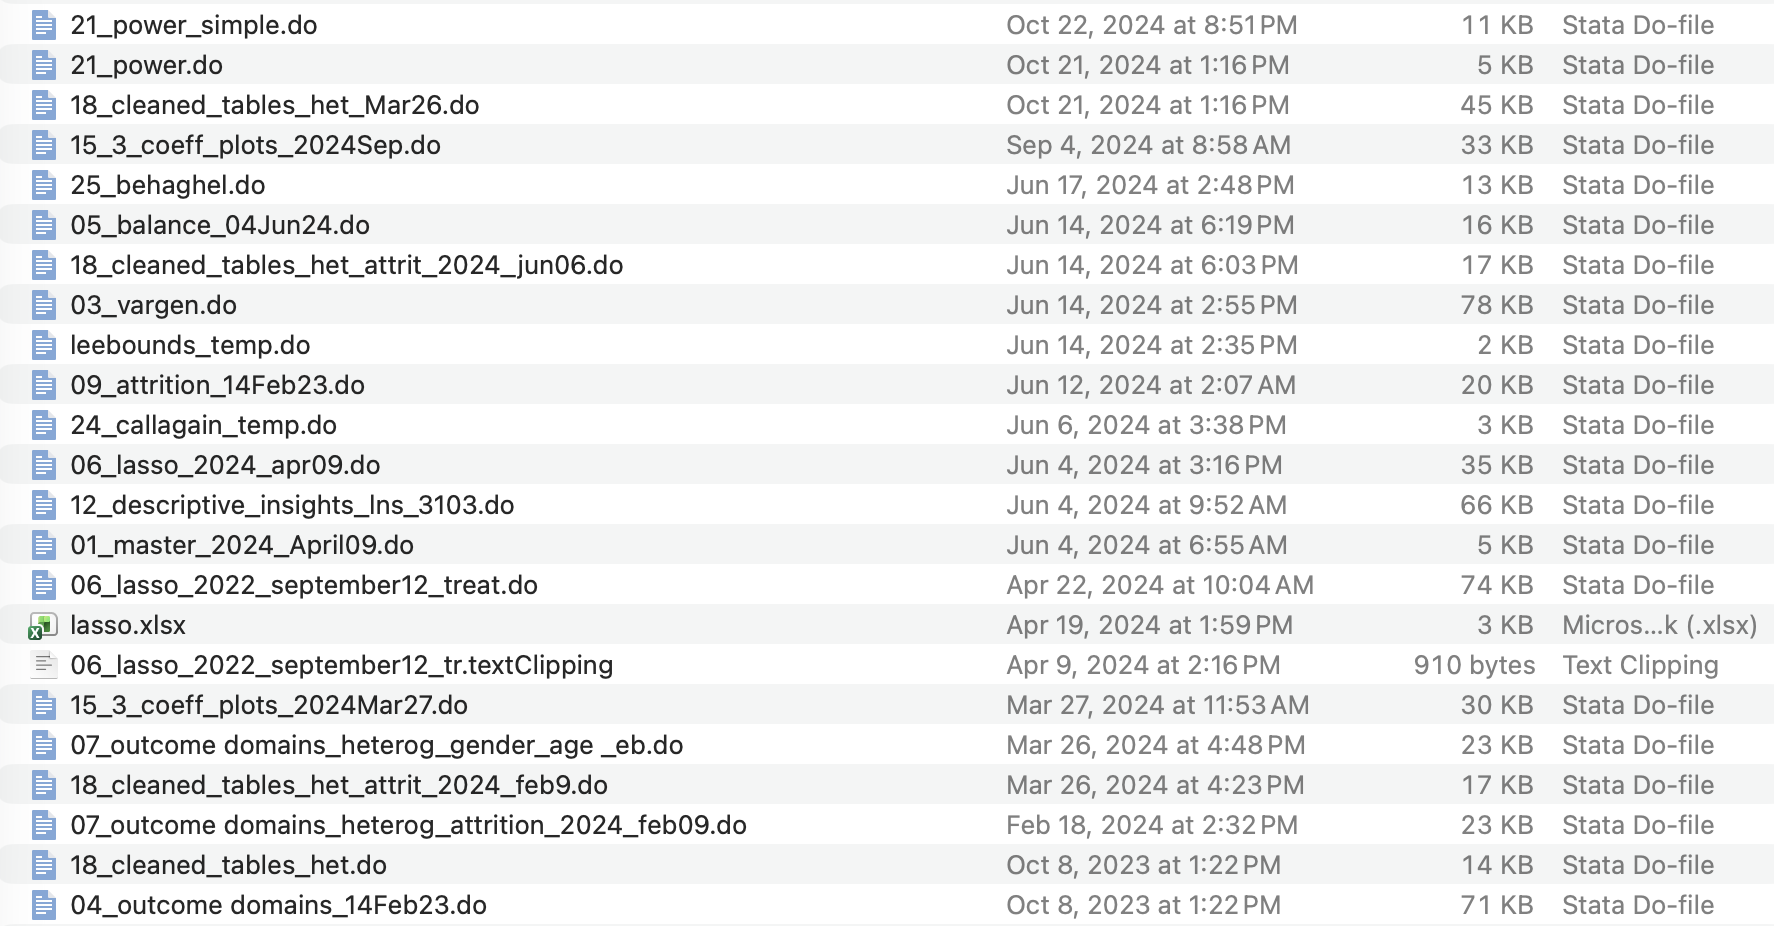
\includegraphics[width=\textwidth, height=0.72\textheight, keepaspectratio]{before_files.png}
\end{column}
\begin{column}{0.45\textwidth}
{\small\color{SoftCoral}\textbf{The problem:} Life happens}
\vskip3pt
\small
\begin{itemize}\setlength{\itemsep}{2pt}
  \item \textbf{51 do-files} across 4 subdirectories
  \item Master file from \textbf{June 2021} --- 5 years stale
  \item Date-in-filename: \texttt{\_07sep}, \texttt{\_02July1130am}
  \item Author-in-filename: \texttt{\_eb}, \texttt{\_e}
  \item No documentation, no version control
\end{itemize}
\vskip3pt
\begin{tcolorbox}[quotebox, top=2pt, bottom=2pt]
\scriptsize This is \textbf{extremely common} in economics.
\end{tcolorbox}
\end{column}
\end{columns}
\end{frame}

%% ====== SLIDE: CODE AUDIT -- THE PROMPT ======
{
\setbeamercolor{background canvas}{bg=DarkSlate}
\begin{frame}[plain]
\centering\vfill
{\color{UVMGold}\faTerminal\quad\fontsize{12}{14}\selectfont THE PROMPT}\\[12pt]
{\fontsize{16}{20}\bfseries\selectfont\color{white} What I Asked Claude to Do}\\[16pt]
\begin{tcolorbox}[colback=DarkSlate!80, colframe=CoolGray!40, boxrule=0.5pt, arc=3pt,
  left=8pt, right=8pt, top=6pt, bottom=6pt, width=12cm]
{\color{white}\ttfamily\scriptsize
Create a clean, replicable version of my do-files that generate the
analysis in my Overleaf paper. I'll give you the file paths.\\[4pt]
Archive all old files --- don't delete anything.\\[4pt]
The goal is a replication package. No results should change.\\[4pt]
Write a comparison script so I can diff the new output against
a ``gold standard'' version from the current code.}
\end{tcolorbox}
\vskip10pt
{\small\color{CoolGray} \faArrowRight\; One prompt. AI reads 51 files, proposes a new structure, archives the old ones, and builds a test harness.}
\vfill
\end{frame}
}

%% ====== SLIDE: CODE AUDIT -- AFTER ======
\begin{frame}{Code Audit: After}
\begin{columns}[T]
\begin{column}{0.50\textwidth}
\centering
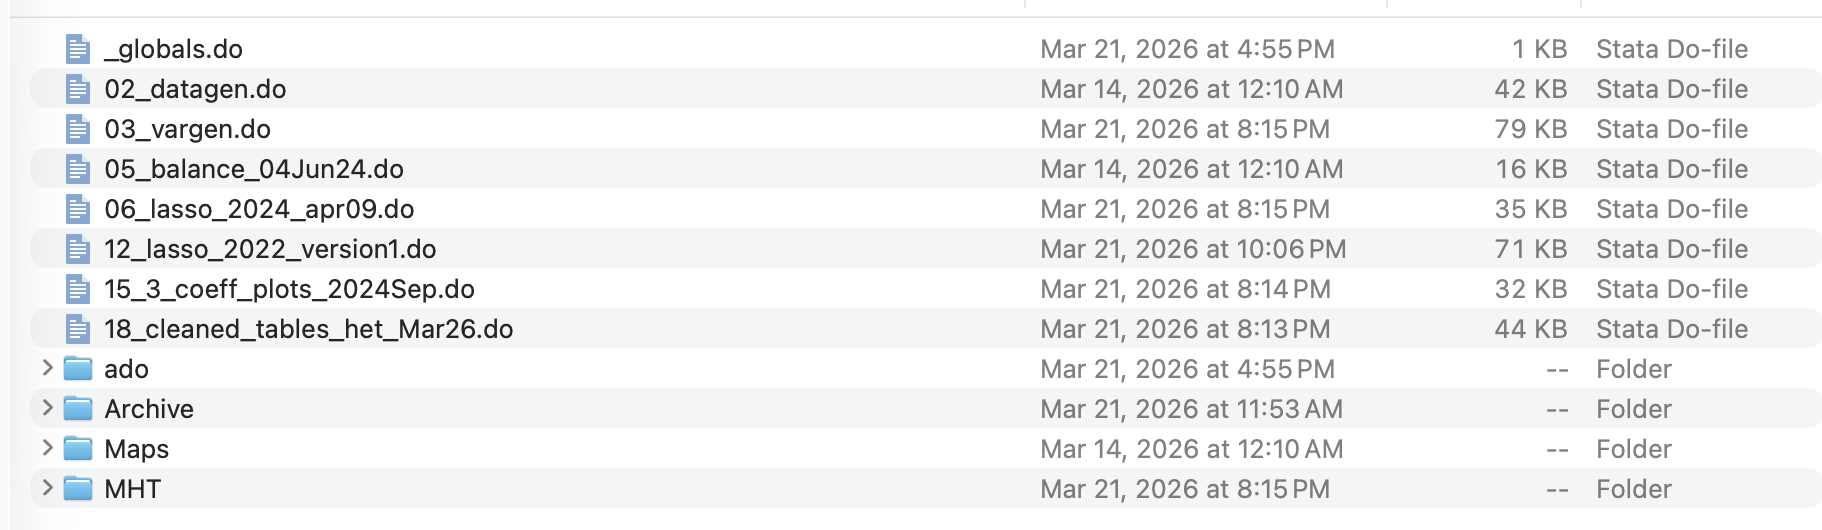
\includegraphics[width=\textwidth, height=0.72\textheight, keepaspectratio]{after_files.png}
\end{column}
\begin{column}{0.45\textwidth}
{\scriptsize
\begin{tabular}{>{\raggedright\arraybackslash}m{2.8cm} >{\centering\arraybackslash}m{1.3cm} >{\centering\arraybackslash}m{1.3cm}}
\rowcolor{SlateTeal}
\textcolor{white}{\textbf{Dimension}} & \textcolor{white}{\textbf{Before}} & \textcolor{white}{\textbf{After}} \\[1pt]
\rowcolor{PaleSage}
Do-files & 51 & \textbf{8} \\[1pt]
\rowcolor{white}
Master file & 2021 & Current \\[1pt]
\rowcolor{PaleSage}
Config system & None & Template \\[1pt]
\rowcolor{white}
Version control & None & Git \\[1pt]
\rowcolor{PaleSage}
Documentation & None & Full \\[1pt]
\end{tabular}
}
\vskip4pt
\begin{tcolorbox}[accentbox, top=2pt, bottom=2pt]
\scriptsize \textbf{86 old variants} preserved in Archive/ --- nothing deleted, fully reversible.
\end{tcolorbox}
\vskip3pt
\begin{tcolorbox}[quotebox, top=2pt, bottom=2pt]
\scriptsize \textbf{Time:} $\sim$2 Claude Code sessions (a few hours).
\textbf{By hand:} days, minimum.
\vskip2pt
\href{file:///Users/ebeam/Dropbox/GitHub/bd-remote-ed/docs/refactoring_audit_2026-03-21.md}{\color{AccentBlue}\faSearch\; \underline{Refactoring audit}}
\;\;
\href{file:///Users/ebeam/Dropbox/GitHub/bd-remote-ed/docs/CHANGELOG.md}{\color{AccentBlue}\faList\; \underline{Changelog}}
\end{tcolorbox}
\end{column}
\end{columns}
\end{frame}

%% ====== SLIDE: THE $FLAGS BUG ======
\begin{frame}[fragile]{The Bug: A Copy-Paste Typo Hiding in Plain Sight}
\vskip-2pt
\begin{tcolorbox}[keybox, title={\faBug\quad The \texttt{\$flags} variable list}, top=2pt, bottom=2pt]
\small
\texttt{\$flags} = 17 missing-value indicators used as controls in \textbf{every regression}. Defined independently in 5 scripts.
\end{tcolorbox}
\vskip3pt
\begin{columns}[T]
\begin{column}{0.47\textwidth}
\begin{tcolorbox}[colback=SoftCoral!8, colframe=SoftCoral, boxrule=0.5pt, arc=2pt, left=5pt, right=5pt, top=3pt, bottom=3pt]
\centering{\small\color{SoftCoral}\textbf{3 of 5 scripts (wrong):}}
\vskip3pt
{\ttfamily\small\color{DeepCharcoal}
... \_f\_c\_engaged \_f\_c\_health\\
\colorbox{SoftCoral!20}{\_c\_child\_work}}
\vskip2pt
{\scriptsize Missing the \texttt{\_f\_} prefix}
\end{tcolorbox}
\end{column}
\begin{column}{0.06\textwidth}
\centering\vskip0.8cm
{\large\color{UVMGold}\faArrowRight}
\end{column}
\begin{column}{0.42\textwidth}
\begin{tcolorbox}[colback=PaleSage, colframe=SlateTeal!50, boxrule=0.5pt, arc=2pt, left=5pt, right=5pt, top=3pt, bottom=3pt]
\centering{\small\color{SlateTeal}\textbf{Correct:}}
\vskip3pt
{\ttfamily\small\color{DeepCharcoal}
... \_f\_c\_engaged \_f\_c\_health\\
\colorbox{PaleSage!50}{\_f\_c\_child\_work}}
\end{tcolorbox}
\end{column}
\end{columns}
\vskip3pt
\begin{tcolorbox}[quotebox, top=2pt, bottom=2pt]
\scriptsize \textbf{Result:} \texttt{\_c\_child\_work} appeared \textit{twice} in regressions. The actual missing indicator was left out. Survived 10+ versions across 2+ years. No error, no crash --- just quietly wrong.
\textbf{How AI found it:} ran \texttt{/code-review} on the new code --- it cross-referenced every \texttt{global flags} definition across all files.
\end{tcolorbox}
\end{frame}

%% ====== SLIDE: /CODE-REVIEW IN ACTION ======
\begin{frame}[fragile]{\texttt{/code-review}: Parallel Agents on the Pipeline}
\begin{columns}[T]
\begin{column}{0.48\textwidth}
\centering
\vskip2pt
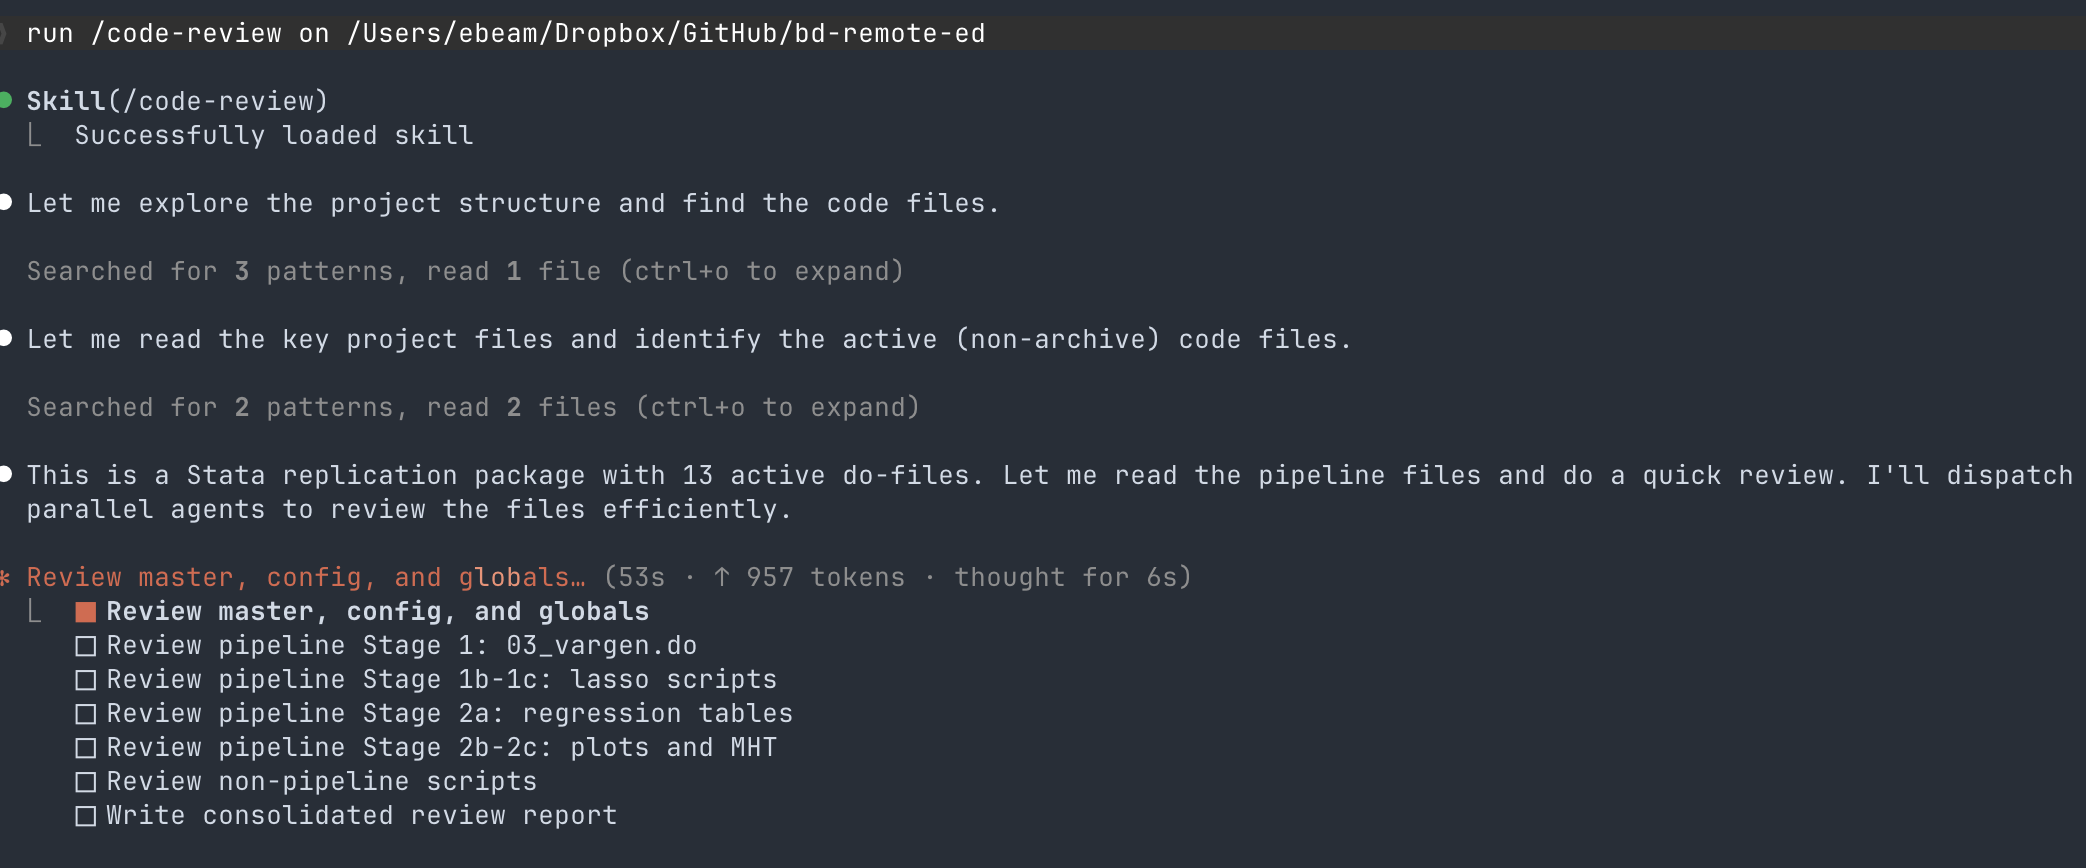
\includegraphics[width=\textwidth, height=0.33\textheight, keepaspectratio]{code_review_launch.png}
\vskip4pt
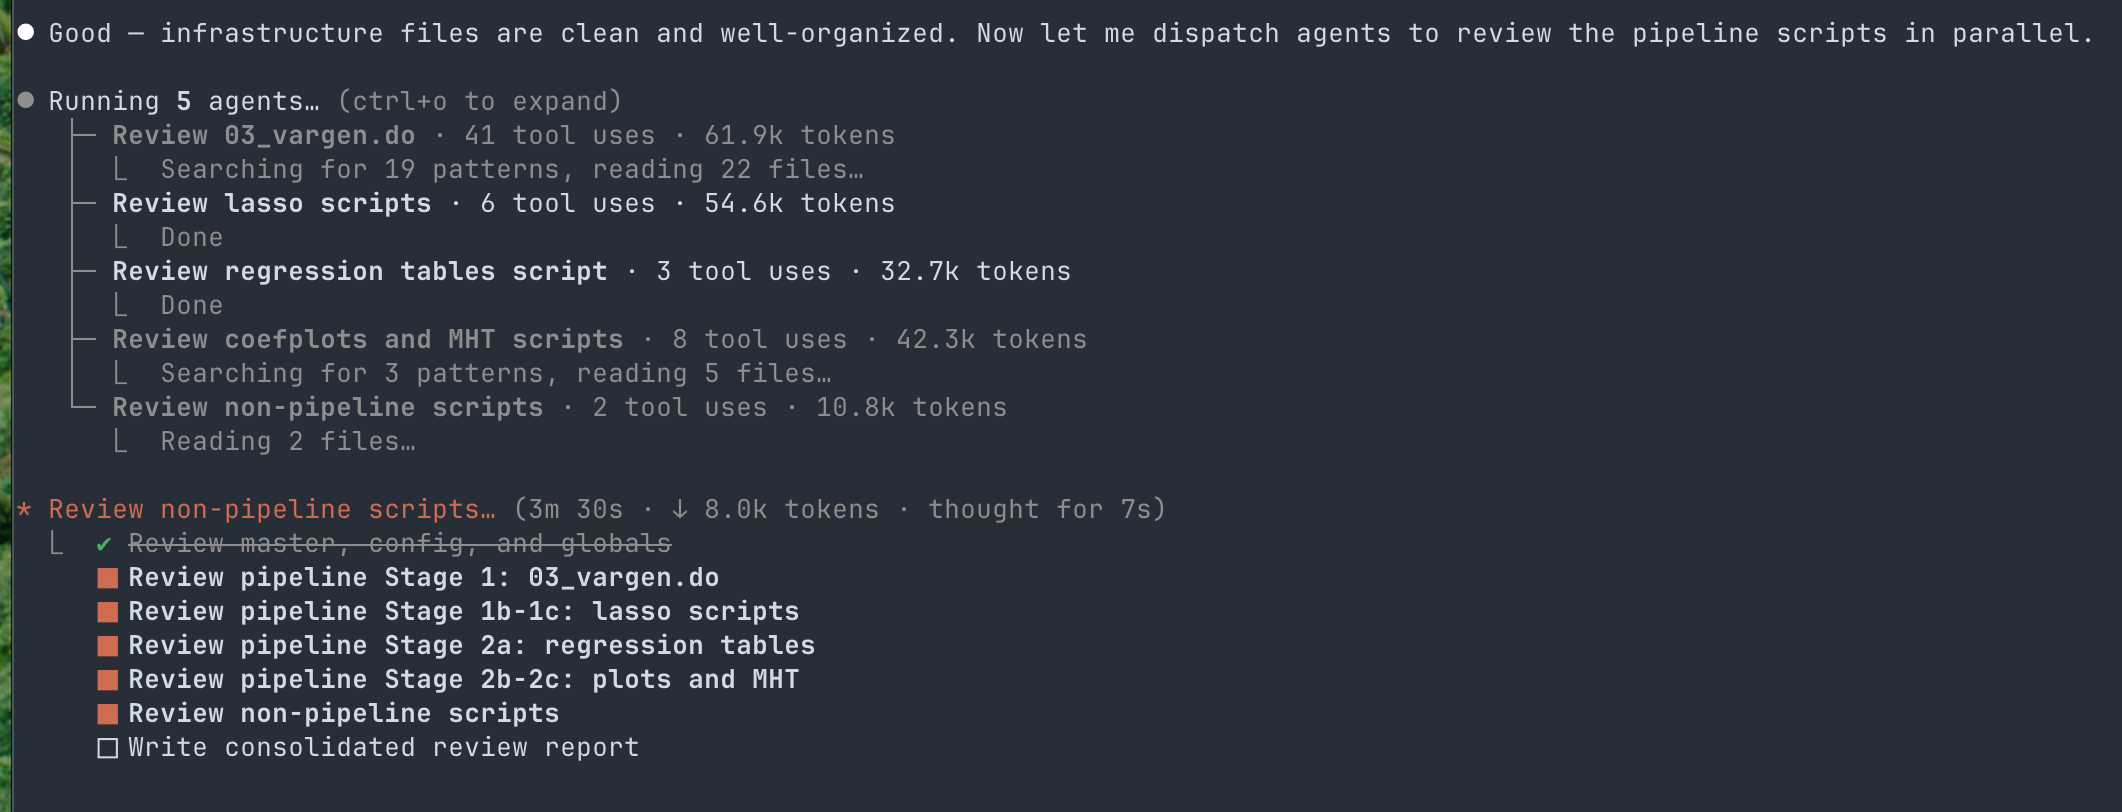
\includegraphics[width=\textwidth, height=0.33\textheight, keepaspectratio]{code_review_agents.png}
\end{column}
\begin{column}{0.46\textwidth}
\begin{tcolorbox}[keybox, title={\faSearch\quad What It Does}]
\scriptsize
\begin{itemize}\setlength{\itemsep}{2pt}
  \item Reads the full pipeline (master $\rightarrow$ all do-files)
  \item Dispatches parallel review agents
  \item Checks correctness, reproducibility, style
  \item Produces a prioritized report
\end{itemize}
\end{tcolorbox}
\vskip4pt
\begin{tcolorbox}[accentbox, top=3pt, bottom=3pt]
\scriptsize
\textbf{This is how it found the \texttt{\$flags} bug} --- cross-referencing every global definition across all files.
\vskip4pt
\href{file:///Users/ebeam/Dropbox/GitHub/bd-remote-ed/code_review_bd-remote-ed_2026-04-26.md}{\color{AccentBlue}\faFile*[regular]\; \underline{Open the full review report}}
\end{tcolorbox}
\end{column}
\end{columns}
\end{frame}

%% ====== SECTION DIVIDER: APP 2 -- PAPER AUDIT ======
{
\setbeamertemplate{footline}{}
\setbeamercolor{background canvas}{bg=SlateTeal}
\begin{frame}[plain, noframenumbering]
\centering\vfill
{\fontsize{22}{28}\bfseries\selectfont\color{white} Application 2}\\[6pt]
{\color{UVMGold}\rule{5cm}{0.8pt}}\\[6pt]
{\normalsize\color{UVMGold} Paper Audit with \texttt{/econ-audit}}\\[4pt]
{\small\color{PaleSage} AI vs.\ 11 Real Referee Reports}
\vfill
\end{frame}
}

%% ====== SLIDE: WHAT IS /ECON-AUDIT ======
\begin{frame}[fragile]{Paper Audit: What Is \texttt{/econ-audit}?}
\vskip-2pt
\begin{columns}[T]
\begin{column}{0.47\textwidth}
\begin{tcolorbox}[keybox, title={\faSearch\quad Adversarial Review Skill}, top=3pt, bottom=3pt]
\small
A reusable skill that reads a paper and acts as a \textbf{skeptical referee}.
\vskip3pt
\begin{itemize}\setlength{\itemsep}{1pt}
  \item Reads full paper (LaTeX, tables, appendix)
  \item Checks identification, power, measurement
  \item Produces structured audit report
  \item Takes $\sim$60 seconds
\end{itemize}
\end{tcolorbox}
\vskip3pt
\begin{tcolorbox}[colback=DarkSlate, colframe=DarkSlate, arc=2pt,
  left=4pt, right=4pt, top=2pt, bottom=2pt]
{\color{CoolGray}\ttfamily\scriptsize \$ npx skills add thinkingwithagents/skills \textbackslash\\
\quad\quad --skill econ-audit}
\end{tcolorbox}
\end{column}
\begin{column}{0.47\textwidth}
\begin{tcolorbox}[accentbox, top=3pt, bottom=3pt]
\small
\textbf{What it checks:}
\vskip3pt
\begin{enumerate}\setlength{\itemsep}{1pt}
  \item \textbf{Identification:} Is the causal claim valid?
  \item \textbf{Statistics:} MHT, power, attrition
  \item \textbf{Measurement:} Are variables measured well?
  \item \textbf{Methodology:} Design consistency
  \item \textbf{Presentation:} Framing, length
\end{enumerate}
\end{tcolorbox}
\end{column}
\end{columns}
\end{frame}

%% ====== SLIDE: LIVE DEMO -- ECON-AUDIT ======
{
\setbeamercolor{background canvas}{bg=DarkSlate}
\begin{frame}[plain]
\centering\vfill
{\color{UVMGold}\faTerminal\quad\fontsize{12}{14}\selectfont LIVE DEMO}\\[12pt]
{\fontsize{18}{22}\bfseries\selectfont\color{white} Running \texttt{/econ-audit} on the Paper}\\[16pt]
\begin{tcolorbox}[colback=DarkSlate!80, colframe=CoolGray!40, boxrule=0.5pt, arc=3pt,
  left=8pt, right=8pt, top=6pt, bottom=6pt, width=11cm]
{\color{CoolGray}\ttfamily\small\$\; claude}\\[4pt]
{\color{white}\ttfamily\small /econ-audit main.tex}
\end{tcolorbox}
\vskip16pt
{\small\color{CoolGray} Reads the full paper + tables + appendix.}\\[4pt]
{\small\color{CoolGray} Produces a structured audit in $\sim$60 seconds.}\\[8pt]
{\small\color{PaleSage} \faPlay\; Switching to terminal\ldots}
\vfill
\end{frame}
}

%% ====== SLIDE: AUDIT RESULTS ======
\begin{frame}[fragile]{\texttt{/econ-audit} Results: After One Pass of Revisions}
\centering
\vskip2pt
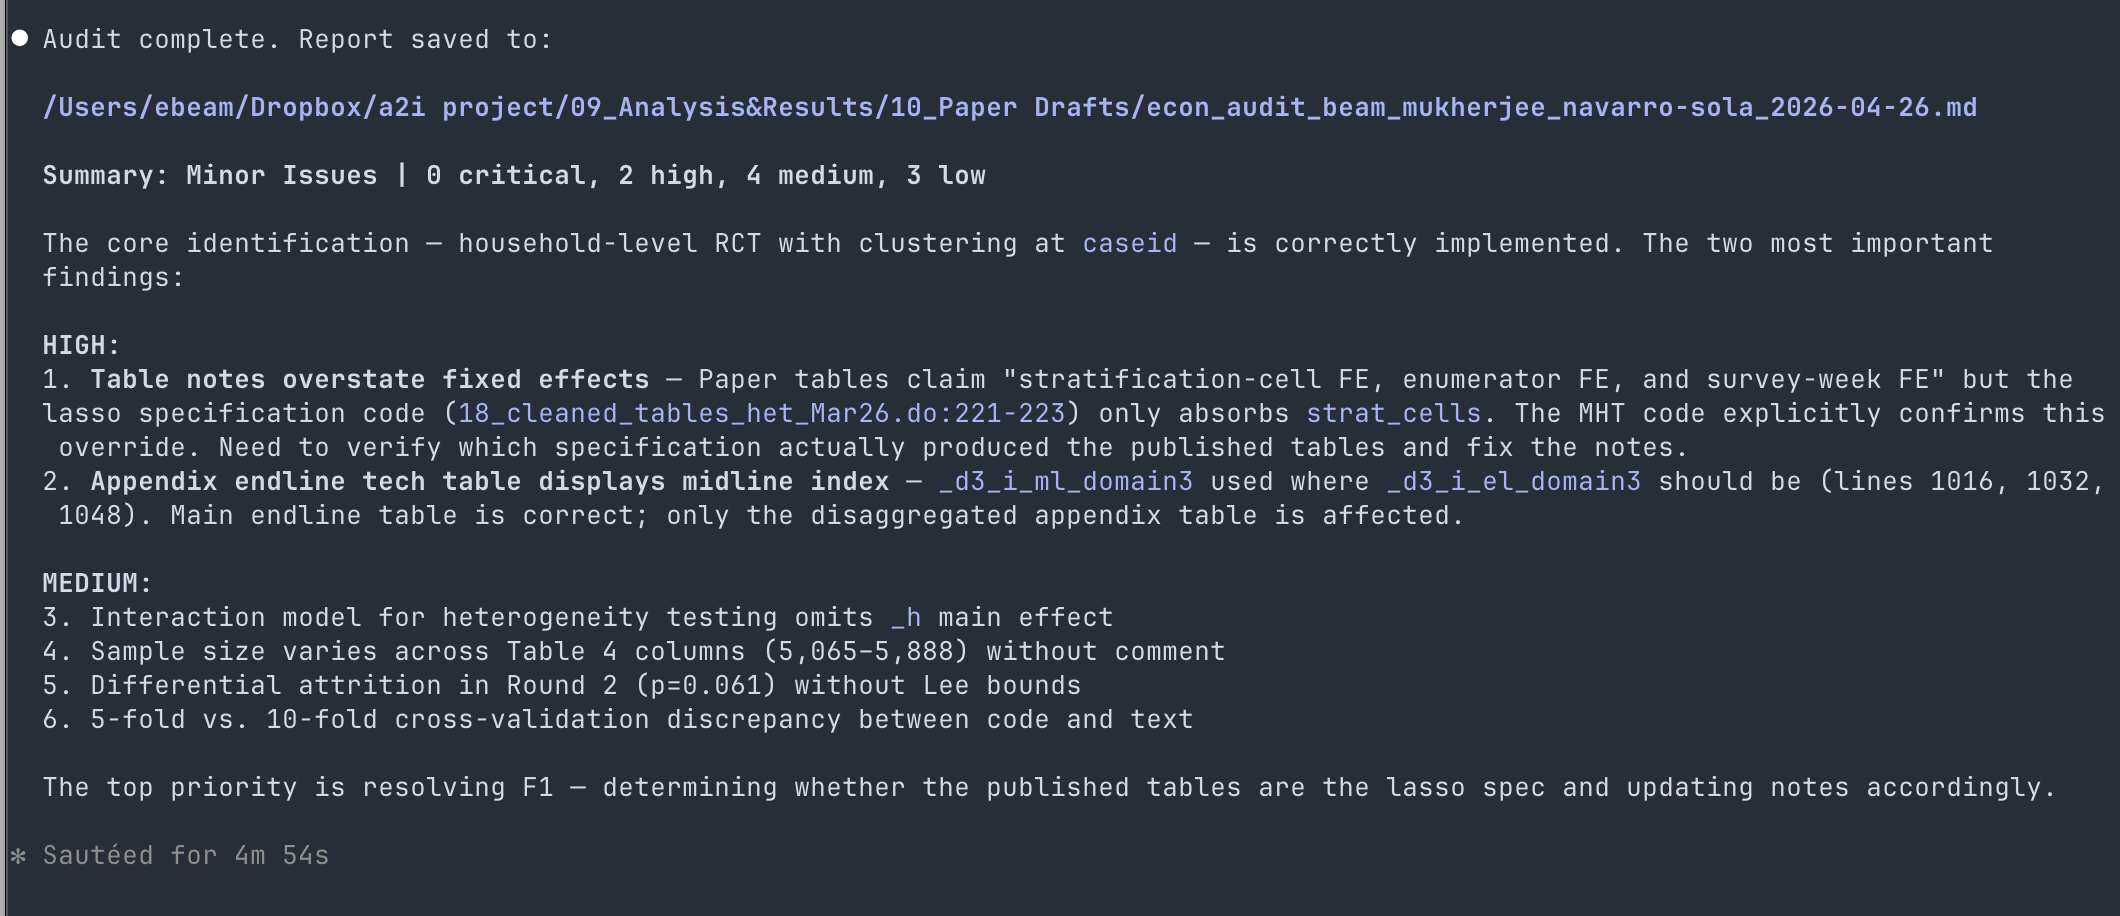
\includegraphics[width=0.92\textwidth, height=0.62\textheight, keepaspectratio]{econ_audit_results.png}
\vskip6pt
\begin{tcolorbox}[accentbox, width=12cm, top=3pt, bottom=3pt]
\small \textbf{0 critical, 2 high, 4 medium, 3 low.} The core identification is correctly implemented. Remaining issues are presentation and robustness.
\end{tcolorbox}
\vskip2pt
{\scriptsize\color{CoolGray}
\href{file:///Users/ebeam/Dropbox/a2i\%20project/09_Analysis\%26Results/10_Paper\%20Drafts/econ_audit_beam_mukherjee_navarro-sola_2026-04-26.md}{\color{AccentBlue}\faFile*[regular]\; \underline{Open the full audit report}}}
\end{frame}

%% ====== SLIDE: AI AUDIT VS REAL REFEREES ======
\begin{frame}{AI Audit vs.\ Real Referees: 7 of 10 in $\sim$60 Seconds}
\vskip-2pt
{\scriptsize
\begin{tabular}{>{\raggedright\arraybackslash}m{5.5cm} c >{\raggedright\arraybackslash}m{5.2cm}}
\rowcolor{SlateTeal}
\textcolor{white}{\textbf{Referee Criticism}} & \textcolor{white}{\textbf{AI?}} & \textcolor{white}{\textbf{Notes}} \\[2pt]
\rowcolor{PaleSage}
High attrition \& differential attrition & \textcolor{SlateTeal}{\faCheck} & Flagged as Critical; suggested Lee bounds \\[2pt]
\rowcolor{white}
Results don't tell a coherent story & \textcolor{UVMGold}{\faAdjust} & Caught ID problem, missed internal contradictions \\[2pt]
\rowcolor{PaleSage}
Theoretical model not useful & \textcolor{SlateTeal}{\faCheck} & Flagged --- but recommended \textit{including} it \\[2pt]
\rowcolor{white}
Short intervention duration (4--8 weeks) & \textcolor{SoftCoral}{\faTimes} & Requires field knowledge \\[2pt]
\rowcolor{PaleSage}
Noisy learning measures (8-item phone test) & \textcolor{SlateTeal}{\faCheck} & Strong match; flagged IRT minimums \\[2pt]
\rowcolor{white}
Paper too long and hard to follow & \textcolor{SlateTeal}{\faCheck} & Suggested cutting 20--30\% \\[2pt]
\rowcolor{PaleSage}
Multiple hypothesis testing issues & \textcolor{SlateTeal}{\faCheck} & Aggressive; added winner's curse framing \\[2pt]
\rowcolor{white}
Limited external validity / COVID fatigue & \textcolor{UVMGold}{\faAdjust} & Partial; missed publication landscape \\[2pt]
\rowcolor{PaleSage}
Deviations from pre-analysis plan & \textcolor{SlateTeal}{\faCheck} & Caught the spirit, not the specifics \\[2pt]
\rowcolor{white}
Complex randomization hard to interpret & \textcolor{SlateTeal}{\faCheck} & Strong match \\[2pt]
\end{tabular}
}
\vskip3pt
\begin{tcolorbox}[accentbox, top=2pt, bottom=2pt, width=12cm]
\centering\small \textbf{5 full matches, 2 partial, 1 opposite recommendation, 2 misses.}\\
11 referee reports across 8 journals over 4 years --- vs.\ 60 seconds of AI.
\end{tcolorbox}
\end{frame}

%% ====== SLIDE: WHAT THE AI MISSED ======
\begin{frame}{What the AI Missed --- And Why It Matters}
\begin{columns}[T]
\begin{column}{0.47\textwidth}
\begin{tcolorbox}[colback=SoftCoral!8, colframe=SoftCoral, boxrule=0.8pt, arc=3pt,
  left=6pt, right=6pt, top=4pt, bottom=4pt,
  fonttitle=\bfseries\small\color{white}, coltitle=white, colbacktitle=SoftCoral,
  title={\faTimes\quad The Misses}]
\small
\begin{itemize}\setlength{\itemsep}{4pt}
  \item \textbf{Short duration:} 4--8 weeks is unusually short for an education RCT. Requires knowing field norms.
  \item \textbf{Internal contradictions:} Data arm increased tutoring \textit{more} than info arm, but only info improved learning. Referees caught this; AI didn't.
  \item \textbf{COVID fatigue:} ``We've seen too many of these papers.'' AI can't know the publication landscape.
\end{itemize}
\end{tcolorbox}
\end{column}
\begin{column}{0.47\textwidth}
\begin{tcolorbox}[quotebox]
\small
\textbf{The opposite advice:}\\[3pt]
The AI recommended \textit{including} the conceptual model. Every referee wanted it \textbf{cut}.
\vskip4pt
Sometimes AI gives exactly the wrong recommendation because it lacks field conventions.
\end{tcolorbox}
\vskip4pt
\begin{tcolorbox}[accentbox]
\small
\textbf{Pattern:}\\[2pt]
AI catches \textbf{statistical/econometric} issues reliably.\\[2pt]
AI misses \textbf{field knowledge}, \textbf{within-paper logic checks}, and \textbf{publication strategy}.
\end{tcolorbox}
\end{column}
\end{columns}
\end{frame}

%% ====== SLIDE: HONEST TAKEAWAY ======
\begin{frame}{Takeaway: A Very Good Pre-Submission Check}
\begin{columns}[T]
\begin{column}{0.50\textwidth}
\begin{tcolorbox}[keybox, title={\faCheck\quad What It Replaces}]
\small
\begin{itemize}\setlength{\itemsep}{3pt}
  \item The first 80\% of what a careful internal seminar discussant would say
  \item Catches the systematic stuff: identification, power, MHT, attrition
  \item In one minute, not one month
\end{itemize}
\end{tcolorbox}
\end{column}
\begin{column}{0.44\textwidth}
\begin{tcolorbox}[colback=SoftCoral!8, colframe=SoftCoral, boxrule=0.5pt, arc=3pt,
  left=6pt, right=6pt, top=4pt, bottom=4pt]
\small
\textbf{What it doesn't replace:}
\vskip3pt
\begin{itemize}\setlength{\itemsep}{2pt}
  \item Field-specific intuition
  \item ``Does this make sense given what we know about Bangladesh?''
  \item Publication strategy advice
  \item Colleagues who know your work
\end{itemize}
\end{tcolorbox}
\end{column}
\end{columns}
\vskip8pt
\begin{tcolorbox}[quotebox, width=13cm]
\small \textbf{For the code audit:} it found bugs I didn't find in two years. That alone justified the time.\\[2pt]
\textbf{For the paper audit:} run it before you send a paper out. It's free. It catches the embarrassing stuff.\\[2pt]
{\scriptsize\color{CoolGray} \textbf{Caveat:} These skills are built for applied micro / dev econ. But they're customizable --- share your own referee reports, successful papers, or field-specific concerns and Claude adapts.}
\end{tcolorbox}
\end{frame}

%% ====== SLIDE: ECON-AUDIT VS REVIEW-PAPER ======
\begin{frame}{\texttt{/econ-audit} vs.\ \texttt{/review-paper}: Zero Overlap}
\vskip-2pt
\begin{columns}[T]
\begin{column}{0.47\textwidth}
\begin{tcolorbox}[keybox, title={\faCode\quad \texttt{/econ-audit} found 6}, top=3pt, bottom=3pt]
\scriptsize
\begin{itemize}\setlength{\itemsep}{1pt}
  \item FE discrepancy in table notes
  \item Wrong index variable in appendix
  \item SES interaction omits main effect
  \item Varying N across Table 4 columns
  \item CV fold discrepancy (5 vs.\ 10)
  \item Missing flag typo (\texttt{\$flags} bug)
\end{itemize}
\vskip2pt
{\tiny\color{CoolGray} All invisible without reading Stata code.}
\end{tcolorbox}
\end{column}
\begin{column}{0.47\textwidth}
\begin{tcolorbox}[colback=LightGold, colframe=UVMGold, boxrule=0.8pt, arc=3pt,
  left=6pt, right=6pt, top=3pt, bottom=3pt,
  fonttitle=\bfseries\small\color{white}, coltitle=white, colbacktitle=UVMGold,
  title={\faFile*[regular]\quad \texttt{/review-paper} found 8}]
\scriptsize
\begin{itemize}\setlength{\itemsep}{1pt}
  \item Attrition severity for learning claim
  \item Marginal significance / $q = 1.000$
  \item Self-reported outcomes during intervention
  \item Mechanism chain is indirect
  \item Mother's income imbalance
  \item Causal language too strong
  \item Cost-effectiveness missing
  \item IRT reliability from short test
\end{itemize}
\vskip2pt
{\tiny\color{CoolGray} All require reading the paper as a referee would.}
\end{tcolorbox}
\end{column}
\end{columns}
\vskip4pt
\begin{tcolorbox}[quotebox, width=13cm, top=2pt, bottom=2pt]
\small \textbf{Zero overlap.} The code audit verifies that the code does what the paper says. The paper review asks whether what the paper says is convincing. \textbf{Run both.}
\end{tcolorbox}
\end{frame}

%% ====== SECTION DIVIDER: APP 3 -- LEE BOUNDS ======
{
\setbeamertemplate{footline}{}
\setbeamercolor{background canvas}{bg=SlateTeal}
\begin{frame}[plain, noframenumbering]
\centering\vfill
{\fontsize{22}{28}\bfseries\selectfont\color{white} Application 3}\\[6pt]
{\color{UVMGold}\rule{5cm}{0.8pt}}\\[6pt]
{\normalsize\color{UVMGold} ``Do Lee Bounds'' --- From Referee Comment to Results}\\[4pt]
{\small\color{PaleSage} Acting on the Audit}
\vfill
\end{frame}
}

%% ====== SLIDE: THE SETUP ======
\begin{frame}{The Referee Said ``Do Lee Bounds''}
\begin{columns}[T]
\begin{column}{0.50\textwidth}
\begin{tcolorbox}[quotebox]
\small
From the AI audit (and real referees):\\[3pt]
``High attrition \& differential attrition. \textbf{Flagged as Critical.} Suggested Lee bounds.''
\vskip4pt
This is the single most common referee request on this paper.
\end{tcolorbox}
\vskip4pt
\begin{tcolorbox}[accentbox, top=3pt, bottom=3pt]
\small
\textbf{The question:} Can AI just\ldots do it?
\vskip2pt
Write the Stata code for Lee (2009) bounds on the \texttt{app} treatment arm vs.\ control?
\end{tcolorbox}
\end{column}
\begin{column}{0.44\textwidth}
\begin{tcolorbox}[keybox, title={\faBook\quad Lee Bounds}]
\scriptsize
\begin{itemize}\setlength{\itemsep}{2pt}
  \item Tightens treatment effect estimates under \textbf{differential attrition}
  \item Trims the ``excess'' group to equalize response rates
  \item Gives upper and lower bounds on the true effect
  \item Standard in development / labor RCTs
\end{itemize}
\end{tcolorbox}
\end{column}
\end{columns}
\end{frame}

%% ====== SLIDE: LIVE DEMO -- LEE BOUNDS ======
{
\setbeamercolor{background canvas}{bg=DarkSlate}
\begin{frame}[plain]
\centering\vfill
{\color{UVMGold}\faTerminal\quad\fontsize{12}{14}\selectfont LIVE DEMO}\\[12pt]
{\fontsize{18}{22}\bfseries\selectfont\color{white} Running Lee Bounds}\\[16pt]
\begin{tcolorbox}[colback=DarkSlate!80, colframe=CoolGray!40, boxrule=0.5pt, arc=3pt,
  left=8pt, right=8pt, top=6pt, bottom=6pt, width=11cm]
{\color{CoolGray}\ttfamily\small\$\; claude}\\[4pt]
{\color{white}\ttfamily\small
I need Lee (2009) bounds for the app treatment arm vs.\ control.
The outcome is the learning index. Use the endline survey flag
to define attrition. Write a Stata do-file, run it, and show me
the upper and lower bounds with confidence intervals.}
\end{tcolorbox}
\vskip12pt
{\small\color{CoolGray} \faArrowRight\; From referee comment to results in one prompt.}
\vfill
\end{frame}
}

%% ====== SLIDE: WHAT JUST HAPPENED ======
\begin{frame}{What Just Happened}
\begin{columns}[T]
\begin{column}{0.47\textwidth}
\begin{tcolorbox}[keybox, title={\faCode\quad AI Wrote the Code}]
\small
\begin{itemize}\setlength{\itemsep}{2pt}
  \item Identified the right variables
  \item Computed attrition rates by arm
  \item Implemented the trimming procedure
  \item Produced bounds with CIs
  \item Formatted a results table
\end{itemize}
\end{tcolorbox}
\end{column}
\begin{column}{0.47\textwidth}
\begin{tcolorbox}[accentbox]
\small
\textbf{What you still check:}
\vskip4pt
\begin{itemize}\setlength{\itemsep}{2pt}
  \item Is the attrition variable right?
  \item Is it trimming from the correct tail?
  \item Do the bounds make sense given your priors?
  \item Does the code match Lee (2009)?
\end{itemize}
\vskip4pt
\textbf{Time:} minutes, not hours.
\end{tcolorbox}
\end{column}
\end{columns}
\vskip6pt
\begin{tcolorbox}[quotebox, width=12cm]
\small The audit flagged it. The AI wrote the code. \textbf{You check the output.} Same principle, end to end.
\end{tcolorbox}
\end{frame}


%% ================================================================
%% ERKMEN'S SECTION: TEACHING & APPLICATIONS
%% ================================================================

%% ====== SECTION DIVIDER: HANDOFF TO ERKMEN ======
{
\setbeamertemplate{footline}{}
\begin{frame}[plain, noframenumbering]
\begin{tikzpicture}[remember picture, overlay]
  \fill[SlateTeal] (current page.north west) rectangle (current page.south east);
  \node[text=white, font=\fontsize{22}{28}\bfseries\selectfont]
    at ([yshift=0.8cm]current page.center) {Erkmen: Teaching \& Applications};
  \draw[UVMGold, line width=0.8pt] ([xshift=-2.5cm, yshift=0.1cm]current page.center) -- ([xshift=2.5cm, yshift=0.1cm]current page.center);
  \node[text=UVMGold, font=\normalsize]
    at ([yshift=-0.5cm]current page.center) {Lecture Builder, Research Brainstorm \& Web Scraping};
\end{tikzpicture}
\end{frame}
}

%% ====== SECTION DIVIDER: APP 3 (Lecture Builder) ======
{
\setbeamertemplate{footline}{}
\begin{frame}[plain, noframenumbering]
\begin{tikzpicture}[remember picture, overlay]
  \fill[SlateTeal] (current page.north west) rectangle (current page.south east);
  \node[text=white, font=\fontsize{22}{28}\bfseries\selectfont]
    at ([yshift=0.4cm]current page.center) {Application 3};
  \node[text=UVMGold, font=\normalsize]
    at ([yshift=-0.4cm]current page.center) {Lecture Builder Skill --- From Papers to a Lecture};
  \draw[UVMGold, line width=0.8pt] ([xshift=-2.5cm, yshift=0cm]current page.center) -- ([xshift=2.5cm, yshift=0cm]current page.center);
\end{tikzpicture}
\end{frame}
}

%% ====== SLIDE: WHERE WE LEFT OFF (the prompt) ======
\begin{frame}[fragile]{Where We Left Off --- The Skill Spec}
\begin{tcolorbox}[promptboxsm]
{\color{CoolGray}\fontsize{6}{7.5}\selectfont\ttfamily /skill-creator\\[2pt]
\color{white}\fontsize{6}{7.5}\selectfont\ttfamily
Create a skill called ``lecture-builder'' that converts academic documents into lecture materials. The skill should:\\[1pt]
1. Read documents in their entirety (PDF, DOCX, web pages) --- break reading into parts to avoid excessive token usage. Include a Python parsing script.\\[1pt]
2. Extract: key arguments, empirical findings, methodological details, discussion points, potential exam questions.\\[1pt]
3. Generate two outputs:\\
\quad a) Structured lecture notes (markdown) with section headers, key takeaways, discussion prompts\\
\quad b) A polished slide deck (draw on \textbackslash academic-beamer-deck or \textbackslash pptx) with clean visuals, one idea per slide\\[1pt]
4. Adapt tone for undergraduate vs.\ graduate audiences (configurable).\\[1pt]
Save SKILL.md + supporting files to .claude/skills/lecture-builder/.
}
\end{tcolorbox}
\vskip3pt
\begin{center}
{\scriptsize\color{CoolGray}\textit{Last week we wrote the spec. \textbf{\color{DeepCharcoal}Today we actually build the skill --- then run it.}}}
\end{center}
\end{frame}

%% ====== SLIDE: BUILDING THE SKILL FLOW ======
\begin{frame}{Building the Skill: \texttt{/skill-creator} Walkthrough}
\centering
\vskip4pt
\begin{tikzpicture}[
  stepbox/.style={
    draw=SlateTeal, fill=PaleSage, rounded corners=3pt,
    minimum width=2.3cm, minimum height=1.2cm,
    align=center, font=\tiny, text=DeepCharcoal
  },
  laststep/.style={
    draw=UVMGold, fill=LightGold, rounded corners=3pt,
    minimum width=2.3cm, minimum height=1.2cm,
    align=center, font=\tiny, text=DeepCharcoal
  },
  arr/.style={-{Stealth[length=3pt]}, SlateTeal, thick}
]
  \node[stepbox] (s1) at (0,0) {{\small\color{SlateTeal}\faTerminal}\\[1pt]\textbf{1. Invoke}\\\texttt{/skill-creator}};
  \node[stepbox, right=0.35cm of s1] (s2) {{\small\color{SlateTeal}\faPaste}\\[1pt]\textbf{2. Paste}\\the spec};
  \node[stepbox, right=0.35cm of s2] (s3) {{\small\color{SlateTeal}\faComments}\\[1pt]\textbf{3. Interview}\\4--6 design Qs};
  \node[stepbox, right=0.35cm of s3] (s4) {{\small\color{SlateTeal}\faCode}\\[1pt]\textbf{4. Skill writes}\\\texttt{SKILL.md} + script};
  \node[laststep, right=0.35cm of s4] (s5) {{\small\color{UVMGold}\faSave}\\[1pt]\textbf{5. Saved}\\\texttt{.claude/skills/}};
  \draw[arr] (s1) -- (s2);
  \draw[arr] (s2) -- (s3);
  \draw[arr] (s3) -- (s4);
  \draw[arr] (s4) -- (s5);
\end{tikzpicture}
\vskip12pt
\pause
\begin{tcolorbox}[accentbox, width=12cm, halign=center]
\scriptsize \texttt{/skill-creator} \textbf{interviews you}. Be ready to answer: name, audience, inputs, outputs, edge cases, where to save.
\end{tcolorbox}
\end{frame}

%% ====== SLIDE: ANATOMY OF THE LECTURE-BUILDER ======
\begin{frame}[fragile]{Anatomy of \texttt{lecture-builder}}
\begin{columns}[T]
\begin{column}{0.55\textwidth}
\centering
\vskip4pt
\begin{tikzpicture}[
  filebox/.style={
    draw=#1, fill=#1!8, rounded corners=2pt,
    minimum width=5.4cm, minimum height=0.55cm,
    align=left, font=\tiny\ttfamily, text=DeepCharcoal
  }
]
  \node[font=\scriptsize\bfseries, text=SlateTeal] at (0,1.9) {\faFolder\; \texttt{.claude/skills/lecture-builder/}};
  \node[filebox=SlateTeal] (skill) at (0,1.2) {\; SKILL.md \hfill {\normalfont\tiny\color{CoolGray}playbook}};
  \node[filebox=UVMGold] (parse) at (0,0.45) {\; parse\_document.py \hfill {\normalfont\tiny\color{CoolGray}PDF/DOCX reader}};
  \node[filebox=AccentBlue] (template) at (0,-0.3) {\; slide\_template.tex \hfill {\normalfont\tiny\color{CoolGray}UVM Beamer}};
  \node[filebox=SoftCoral] (notes) at (0,-1.05) {\; notes\_template.md \hfill {\normalfont\tiny\color{CoolGray}notes scaffold}};
\end{tikzpicture}
\end{column}
\begin{column}{0.42\textwidth}
\vskip4pt
\begin{tcolorbox}[keybox, title={What \texttt{SKILL.md} enforces}]
\scriptsize
\begin{itemize}\setlength{\itemsep}{1pt}
  \item Chunked reading $\rightarrow$ token control
  \item Mandatory citations from source PDFs
  \item Undergrad vs.\ grad tone toggle
  \item Dual output: notes + slides
  \item Reuses UVM color palette
\end{itemize}
\end{tcolorbox}
\end{column}
\end{columns}
\vskip4pt
\pause
\begin{tcolorbox}[quotebox, width=12cm]
\scriptsize Skills with Python scripts $>$ pure-markdown skills when tokens matter. The script reads; the LLM synthesizes.
\end{tcolorbox}
\end{frame}

%% ====== SLIDE: THE INPUT FOLDER ======
\begin{frame}{The Input Folder}
\begin{columns}[T]
\begin{column}{0.46\textwidth}
\centering
\vskip4pt
\begin{tikzpicture}[
  pdfbox/.style={
    draw=SlateTeal, fill=PaleSage, rounded corners=2pt,
    minimum width=5cm, minimum height=0.8cm,
    align=left, font=\scriptsize, text=DeepCharcoal
  },
  folderbox/.style={
    draw=UVMGold, fill=LightGold, rounded corners=3pt,
    minimum width=5.6cm, minimum height=0.55cm,
    align=center, font=\scriptsize\bfseries, text=DeepCharcoal
  }
]
  \node[folderbox] (fold) at (0,2.1) {\faFolderOpen\; \texttt{./inputs/}};
  \node[pdfbox] (p1) at (0,1.1) {\;\faFilePdf\; \texttt{gov\_thinktank\_ice\_arrests.pdf}\\[-1pt]\hspace*{1.4em}{\tiny\color{CoolGray} policy report}};
  \node[pdfbox] (p2) at (0,0.0) {\;\faFilePdf\; \texttt{ice\_enforcement\_report.pdf}\\[-1pt]\hspace*{1.4em}{\tiny\color{CoolGray} government brief}};
  \node[pdfbox] (p3) at (0,-1.1) {\;\faFilePdf\; \texttt{aslim\_paper.pdf}\\[-1pt]\hspace*{1.4em}{\tiny\color{CoolGray} academic working paper}};
  \draw[-{Stealth[length=3pt]}, CoolGray] (fold.south) -- ($(fold.south)+(0,-0.18)$);
\end{tikzpicture}
\end{column}
\begin{column}{0.50\textwidth}
\vskip4pt
\begin{tcolorbox}[accentbox]
\scriptsize
\textbf{Why this mix?}
\vskip3pt
\begin{itemize}\setlength{\itemsep}{1pt}
  \item Heterogeneous sources: \textbf{policy} + \textbf{government} + \textbf{academic}
  \item Forces the skill to harmonize tone, terminology, and evidence quality
  \item Mirrors how you'd actually build a lecture
\end{itemize}
\end{tcolorbox}
\vskip4pt
\pause
\begin{tcolorbox}[quotebox]
\scriptsize \textbf{Topic:} The labor and health consequences of ICE enforcement. Connects directly to ongoing research at UVM.
\end{tcolorbox}
\end{column}
\end{columns}
\end{frame}

%% ====== SLIDE: EXECUTION PROMPT ======
\begin{frame}[fragile]{The Execution Prompt}
\begin{tcolorbox}[promptboxsm]
{\color{CoolGray}\fontsize{5.5}{7}\selectfont\ttfamily /lecture-builder\\[2pt]
\color{white}\fontsize{5.5}{7}\selectfont\ttfamily
I have a folder ./inputs/ with: gov\_thinktank\_ice\_arrests.pdf,\\
ice\_enforcement\_report.pdf, aslim\_paper.pdf.\\[2pt]
Build a 50-minute undergraduate lecture on the labor and health\\
consequences of ICE enforcement. Audience: junior/senior econ majors\\
who have taken intermediate micro and one applied econometrics class.\\[2pt]
Outputs to ./outputs/:\\
\hspace*{1em}1) lecture\_notes.md --- sectioned notes with 5 key takeaways,\\
\hspace*{2em}4 discussion prompts, 3 candidate exam questions.\\
\hspace*{1em}2) lecture\_slides.tex --- Beamer deck (\textasciitilde 20 slides, 16:9). Use\\
\hspace*{2em}a clean academic palette --- default UVM (deep green / gold) or ask\\
\hspace*{2em}me. In-text citations to all three source PDFs.\\[2pt]
Be conservative with tokens: parse each PDF in chunks via\\
parse\_document.py, summarize per-section, then synthesize.
}
\end{tcolorbox}
\vskip3pt
\begin{center}
{\scriptsize\color{CoolGray}\textit{Audience spec + output spec + token discipline. Skills work better when the prompt is concrete.}}
\end{center}
\end{frame}

%% ====== SLIDE: EXPECTED OUTPUT ======
\begin{frame}{Expected Output (Live Demo Running)}
\centering
\vskip2pt
\begin{tcolorbox}[accentbox, width=11cm, halign=center, top=3pt, bottom=3pt]
\scriptsize \faPlay\quad Live demo running in the background --- final files appear by the end of this section
\end{tcolorbox}
\vskip6pt
\begin{tikzpicture}[
  doc/.style={
    draw=CoolGray!50, fill=white, rounded corners=2pt,
    minimum width=5cm, minimum height=4cm, align=left, font=\tiny,
    inner sep=4pt
  }
]
  \node[doc] (notes) at (-3.2,0) {%
    \textbf{lecture\_notes.md}\\[2pt]
    \rule{4.4cm}{0.3pt}\\[1pt]
    {\color{SlateTeal}\bfseries\# 1. The setting}\\
    Recent expansions of interior immigration\\
    enforcement\ldots\\[1pt]
    {\color{SlateTeal}\bfseries\# 2. Identification strategy}\\
    287(g) rollout as a staggered DiD\ldots\\[1pt]
    {\color{SlateTeal}\bfseries\# 3. Findings}\\
    Aslim et al.\ document\ldots\\[1pt]
    {\color{UVMGold}\bfseries\# Discussion prompts}\\
    1. Why might the effect on infant\\
    \hspace*{1em}health attenuate over time?\\[1pt]
    {\color{UVMGold}\bfseries\# Exam questions}\\
    1. Sketch the parallel-trends test\ldots
  };
  \node[doc] (slides) at (3.2,0) {%
    \textbf{lecture\_slides.tex}\\[2pt]
    \rule{4.4cm}{0.3pt}\\[1pt]
    {\color{CoolGray}\% 20 slides, 16:9}\\
    {\color{CoolGray}\% UVM palette}\\[2pt]
    \texttt{\textbackslash begin\{frame\}\{Setting\}}\\
    \hspace*{1em}\faChartBar\; ICE arrests timeline\\
    \texttt{\textbackslash end\{frame\}}\\[2pt]
    \texttt{\textbackslash begin\{frame\}\{Methods\}}\\
    \hspace*{1em}\faCogs\; staggered DiD\\
    \texttt{\textbackslash end\{frame\}}\\[2pt]
    \texttt{\textbackslash begin\{frame\}\{Results\}}\\
    \hspace*{1em}\faChartLine\; main effect\\
    \texttt{\textbackslash end\{frame\}}
  };
  \draw[-{Stealth[length=3pt]}, UVMGold, thick] (notes.east) -- (slides.west) node[midway, above, font=\tiny, text=CoolGray] {synthesizes};
\end{tikzpicture}
\end{frame}

%% ====== SLIDE: WHAT JUST HAPPENED ======
\begin{frame}{What Just Happened (Under the Hood)}
\centering
\vskip4pt

\begin{tikzpicture}[
  stage/.style={
    draw=SlateTeal, fill=PaleSage, rounded corners=4pt,
    minimum width=3cm, minimum height=1.6cm,
    align=center, font=\scriptsize, text=DeepCharcoal
  },
  arr/.style={-{Stealth[length=4pt]}, UVMGold, thick}
]
  \node<1->[stage] (read) at (-4.8,0)
    {{\large\color{SlateTeal}\faFilePdf}\\[2pt]\textbf{Read in chunks}\\{\tiny parse\_document.py}};
  \node<2->[stage] (synth) at (0,0)
    {{\large\color{SlateTeal}\faBrain}\\[2pt]\textbf{Synthesize}\\{\tiny LLM does the writing}};
  \node<3->[stage] (render) at (4.8,0)
    {{\large\color{SlateTeal}\faPalette}\\[2pt]\textbf{Render}\\{\tiny notes + Beamer .tex}};
  \draw<2->[arr] (read) -- (synth);
  \draw<3->[arr] (synth) -- (render);
\end{tikzpicture}
\vskip12pt
\onslide<4->{%
\begin{tcolorbox}[quotebox, width=11cm]
\scriptsize \textbf{This skill is reusable.} Swap the input folder, swap the topic, swap the audience --- get a new lecture in minutes. Build once, deploy forever.
\end{tcolorbox}%
}
\end{frame}

%% ====== SECTION DIVIDER: APP 4 ======
{
\setbeamertemplate{footline}{}
\begin{frame}[plain, noframenumbering]
\begin{tikzpicture}[remember picture, overlay]
  \fill[SlateTeal] (current page.north west) rectangle (current page.south east);
  \node[text=white, font=\fontsize{22}{28}\bfseries\selectfont]
    at ([yshift=0.4cm]current page.center) {Application 4};
  \node[text=UVMGold, font=\normalsize]
    at ([yshift=-0.4cm]current page.center) {\texttt{/research-brainstorm} --- Stress-Test a Research Idea};
  \draw[UVMGold, line width=0.8pt] ([xshift=-2.5cm, yshift=0cm]current page.center) -- ([xshift=2.5cm, yshift=0cm]current page.center);
\end{tikzpicture}
\end{frame}
}

%% ====== SLIDE: WHAT THE BRIEF CONTAINS ======
\begin{frame}{What the Research Brief Contains}
\begin{columns}[T]
\begin{column}{0.55\textwidth}
\begin{tcolorbox}[keybox, title={\faFile\quad Brief sections}, width=\textwidth]
\scriptsize
\begin{itemize}\setlength{\itemsep}{1pt}
  \item \textbf{The question} --- structured: unit, population, treatment, outcome, comparison, setting
  \item \textbf{Closest related work} --- 3--6 cites with sharp delta
  \item \textbf{Contribution type} --- setting / identification / reframing / measurement / mechanism / policy
  \item \textbf{The strongest objection} --- one paragraph, unvarnished
  \item \textbf{Alternative framings} --- 2--3 pivots
  \item \textbf{Feasibility} --- data, identification, power, timeline, fatal risks
  \item \textbf{Next concrete step}
\end{itemize}
\end{tcolorbox}
\end{column}
\begin{column}{0.42\textwidth}
\vskip2pt
\begin{tcolorbox}[accentbox]
\scriptsize
\textbf{Saved to:}\\
{\tiny\ttfamily research\_briefs/YYYY-MM-DD-{slug}.md}
\vskip4pt
Markdown so it lives next to your other notes. Re-openable, editable, citeable in your own write-ups.
\end{tcolorbox}
\vskip6pt
\pause
\begin{tcolorbox}[quotebox]
\scriptsize \textit{The conversation is great.\\ The artifact is what you keep.}
\end{tcolorbox}
\end{column}
\end{columns}
\end{frame}

%% ====== SLIDE: INSTALLING IT ======
\begin{frame}[fragile]{Installing \texttt{/research-brainstorm}}
\begin{columns}[T]
\begin{column}{0.48\textwidth}
\begin{tcolorbox}[keybox, title={\faCubes\quad Full economist pack}]
\scriptsize
{\tiny\ttfamily npx skills add\\\hspace*{1em}thinkingwithagents/skills}
\vskip4pt
Installs the full pack in one go. Today we use: {\fontsize{6.5}{8}\selectfont\ttfamily research-brainstorm, find-data, academic-beamer-deck.}
\end{tcolorbox}
\end{column}
\begin{column}{0.48\textwidth}
\begin{tcolorbox}[keybox, title={\faPuzzlePiece\quad One skill at a time}]
\scriptsize
{\tiny\ttfamily npx skills add\\\hspace*{1em}thinkingwithagents/skills\\\hspace*{1em}-{}-skill research-brainstorm}
\vskip4pt
Mix-and-match per project. Lighter footprint when you only need one.
\end{tcolorbox}
\end{column}
\end{columns}
\vskip6pt
\pause
\begin{tcolorbox}[accentbox, width=12cm, halign=center, top=3pt, bottom=3pt]
\scriptsize Same \texttt{npx skills} mechanism works for any GitHub-hosted skill repo. \textbf{Build your own pack and share it with your coauthors.}
\end{tcolorbox}
\end{frame}

%% ====== SLIDE: LIVE DEMO -- BRING ME A QUESTION ======
\begin{frame}{Live Demo: Hand Me a Question}
\centering
\vskip4pt
\begin{tcolorbox}[colback=SlateTeal, colframe=SlateTeal, arc=4pt, width=11cm, halign=center, top=8pt, bottom=8pt]
{\color{white}\Large\bfseries Audience:}\\[3pt]
{\color{UVMGold}\large\itshape hand me a half-formed research question.}
\end{tcolorbox}
\vskip10pt
\pause
\begin{columns}[T]
\begin{column}{0.31\textwidth}
\begin{tcolorbox}[quotebox, top=3pt, bottom=3pt]
\scriptsize\centering
\textbf{An effect}\\you suspect\\but can't yet measure
\end{tcolorbox}
\end{column}
\begin{column}{0.31\textwidth}
\begin{tcolorbox}[quotebox, top=3pt, bottom=3pt]
\scriptsize\centering
\textbf{A dataset}\\you have access to\\but haven't used
\end{tcolorbox}
\end{column}
\begin{column}{0.31\textwidth}
\begin{tcolorbox}[quotebox, top=3pt, bottom=3pt]
\scriptsize\centering
\textbf{A policy}\\you want\\to evaluate
\end{tcolorbox}
\end{column}
\end{columns}
\vskip8pt
{\scriptsize\color{CoolGray} Live: invoke \texttt{/research-brainstorm}, ride through the phases, walk away with a brief.}
\end{frame}

%% ====== SECTION DIVIDER: APP 5 ======
{
\setbeamertemplate{footline}{}
\begin{frame}[plain, noframenumbering]
\begin{tikzpicture}[remember picture, overlay]
  \fill[SlateTeal] (current page.north west) rectangle (current page.south east);
  \node[text=white, font=\fontsize{22}{28}\bfseries\selectfont]
    at ([yshift=0.4cm]current page.center) {Application 5};
  \node[text=UVMGold, font=\normalsize]
    at ([yshift=-0.4cm]current page.center) {Web Scraper --- From \texttt{/find-data} to a Live Visualization};
  \draw[UVMGold, line width=0.8pt] ([xshift=-2.5cm, yshift=0cm]current page.center) -- ([xshift=2.5cm, yshift=0cm]current page.center);
\end{tikzpicture}
\end{frame}
}

%% ====== SLIDE: APP 5 -- BRIEF FIND-DATA SLIDE ======
\begin{frame}{\texttt{/find-data} Picks NBER Working Papers}
\begin{columns}[T]
\begin{column}{0.46\textwidth}
\begin{tcolorbox}[keybox, title={\faSearch\quad \texttt{/find-data} in one line}]
\scriptsize
We hand it our constraints (applied-micro audience, 24+ months, scrape-able, time-series + cross-section). It scans repositories and surfaces a source.
\vskip3pt
\textbf{Today's pick:} NBER working papers.
\end{tcolorbox}
\end{column}
\begin{column}{0.50\textwidth}
\begin{tcolorbox}[accentbox]
\scriptsize
\textbf{Why NBER:} every economist cares; clean HTML; rich JEL + affiliation cross-section; \textasciitilde 1{,}500 papers / year.
\vskip3pt
\textbf{URL:}\\
{\tiny\ttfamily nber.org/papers?page=N\&perPage=100\&sortBy=public\_date}
\vskip3pt
\textbf{Extract:} {\fontsize{6.5}{8}\selectfont\ttfamily nber\_number, title, authors, public\_date, primary\_jel\_code, affiliations.}
\end{tcolorbox}
\end{column}
\end{columns}
\vskip4pt
\begin{center}
{\scriptsize\color{CoolGray}\textit{Goal: novel data on the screen in under 10 minutes. Skip the buildup --- go straight to scraping.}}
\end{center}
\end{frame}

%% ====== SLIDE: INSPECT THE PAGE ======
\begin{frame}{Inspect Before You Prompt}
\centering
\vskip2pt
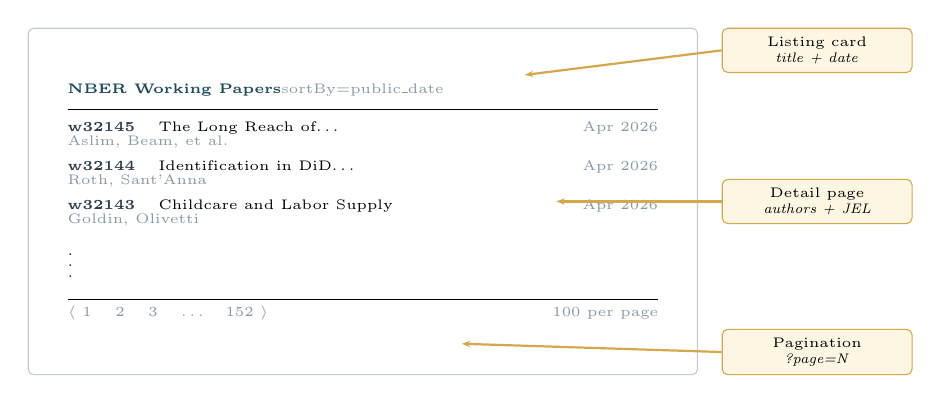
\begin{tikzpicture}[
  page/.style={
    draw=CoolGray!50, fill=white, rounded corners=2pt,
    minimum width=8.5cm, minimum height=4.4cm, font=\tiny,
    align=left, inner sep=6pt
  },
  callout/.style={
    draw=UVMGold, fill=LightGold, rounded corners=2pt,
    font=\tiny, align=center, inner sep=3pt
  },
  arr/.style={-{Stealth[length=3pt]}, UVMGold, thick}
]
  \node[page] (p) at (0,0) {%
    {\color{SlateTeal}\bfseries NBER Working Papers}\hfill {\tiny\color{CoolGray}sortBy=public\_date}\\
    \rule{7.5cm}{0.3pt}\\[2pt]
    {\color{DeepCharcoal}\bfseries w32145} \;\; The Long Reach of\ldots \hfill {\tiny\color{CoolGray}Apr 2026}\\[-1pt]
    {\tiny\color{CoolGray} Aslim, Beam, et al.}\\[3pt]
    {\color{DeepCharcoal}\bfseries w32144} \;\; Identification in DiD\ldots \hfill {\tiny\color{CoolGray}Apr 2026}\\[-1pt]
    {\tiny\color{CoolGray} Roth, Sant'Anna}\\[3pt]
    {\color{DeepCharcoal}\bfseries w32143} \;\; Childcare and Labor Supply\hfill {\tiny\color{CoolGray}Apr 2026}\\[-1pt]
    {\tiny\color{CoolGray} Goldin, Olivetti}\\[3pt]
    \vdots\\[2pt]
    \rule{7.5cm}{0.3pt}\\
    {\tiny\color{CoolGray}$\langle$ 1 \;\; 2 \;\; 3 \;\; \ldots \;\; 152 $\rangle$ \hfill 100 per page}
  };
  % Callouts
  \node[callout, right=0.3cm of p.north east, anchor=north west, text width=2.2cm] (c1) {Listing card\\\textit{title + date}};
  \node[callout, right=0.3cm of p.east, anchor=west, text width=2.2cm] (c2) {Detail page\\\textit{authors + JEL}};
  \node[callout, right=0.3cm of p.south east, anchor=south west, text width=2.2cm] (c3) {Pagination\\\textit{?page=N}};
  \draw[arr] (c1.west) -- ($(p.north east)+(-2.2,-0.6)$);
  \draw[arr] (c2.west) -- ($(p.east)+(-1.8,0)$);
  \draw[arr] (c3.west) -- ($(p.south east)+(-3,0.4)$);
\end{tikzpicture}
\vskip4pt
{\scriptsize\color{CoolGray}\textit{View-source first.} The agent writes better scrapers when you've already named the selectors.}
\end{frame}

%% ====== SLIDE: SCRAPING PROMPT ======
\begin{frame}[fragile]{The Scraping Prompt}
\begin{tcolorbox}[promptboxsm]
{\color{white}\fontsize{5.5}{7}\selectfont\ttfamily
Scrape NBER working papers for a teaching demo. Build a self-contained\\
Python script in ./scrape\_nber/ using uv:\\[2pt]
1.\;Fetch the most recent \textasciitilde 1{,}000 papers from\\
\hspace*{1.5em}nber.org/papers?page=N\&perPage=100\&sortBy=public\_date\\
\hspace*{1.5em}(paginate until 1{,}000 or cutoff 2024-01-01).\\
2.\;Extract: nber\_number, title, authors, public\_date, primary\\
\hspace*{1.5em}JEL code, affiliations (from detail page if needed).\\
3.\;Save to ./scrape\_nber/data/nber\_papers.csv.\\
4.\;Generate three PNGs to ./scrape\_nber/figures/:\\
\hspace*{1.5em}- papers\_per\_month.png \quad bars, last 24 months, UVM colors\\
\hspace*{1.5em}- top\_jel\_codes.png \quad top 15 primary JEL codes\\
\hspace*{1.5em}- top\_institutions.png \quad top 10 affiliations\\
5.\;Print 5-line stdout summary.\\[2pt]
Politeness: real-browser User-Agent; sleep 0.5s between fetches;\\
cache HTML to ./scrape\_nber/cache/ so re-runs are free.
}
\end{tcolorbox}
\end{frame}

%% ====== SLIDE: WHAT THE AGENT DOES ======
\begin{frame}{What Claude Does While We Keep Talking}
\begin{columns}[T]
\begin{column}{0.42\textwidth}
\centering
\vskip4pt
\begin{tikzpicture}[
  stage/.style={
    draw=CoolGray!50, fill=PaleSage, rounded corners=3pt,
    minimum width=4.2cm, minimum height=0.85cm,
    align=center, font=\scriptsize, text=DeepCharcoal
  },
  active/.style={
    draw=UVMGold, fill=LightGold, rounded corners=3pt,
    minimum width=4.2cm, minimum height=0.85cm,
    align=center, font=\scriptsize\bfseries, text=DeepCharcoal
  }
]
  \only<1>{\node[active] (s1) at (0,1.2) {\faSpinner\quad Fetching pages\ldots};}
  \only<2->{\node[stage] (s1) at (0,1.2) {\color{SlateTeal}\faCheck\quad Fetched 10 / 10 pages};}
  \only<-1>{\node[stage] (s2) at (0,0) {\color{CoolGray} Parsing\ldots};}
  \only<2>{\node[active] (s2) at (0,0) {\faSpinner\quad Parsing 1{,}000 records\ldots};}
  \only<3->{\node[stage] (s2) at (0,0) {\color{SlateTeal}\faCheck\quad Parsed 1{,}000 records};}
  \only<-2>{\node[stage] (s3) at (0,-1.2) {\color{CoolGray} Plotting\ldots};}
  \only<3>{\node[active] (s3) at (0,-1.2) {\faSpinner\quad Plotting 3 figures\ldots};}
  \only<4->{\node[stage] (s3) at (0,-1.2) {\color{SlateTeal}\faCheck\quad Wrote 3 PNGs};}
\end{tikzpicture}
\end{column}
\begin{column}{0.54\textwidth}
\vskip4pt
\begin{tcolorbox}[colback=DarkSlate, colframe=DarkSlate, arc=2pt, left=6pt, right=6pt, top=4pt, bottom=4pt]
{\color{white}\ttfamily\tiny
\$ uv run scrape\_nber/main.py\\[1pt]
{\color{CoolGray}[INFO]} fetching page 1/10 \ldots ok (98 papers)\\
{\color{CoolGray}[INFO]} fetching page 2/10 \ldots ok (100 papers)\\
{\color{CoolGray}[INFO]} \ldots\\
{\color{CoolGray}[INFO]} parsing JEL codes \ldots\\
{\color{CoolGray}[INFO]} saved data/nber\_papers.csv\\
{\color{CoolGray}[INFO]} writing figures/\ldots\\[3pt]
{\color{UVMGold}== Summary ==}\\
{\color{white}n\_papers: 1{,}000}\\
{\color{white}date range: 2024-04 to 2026-04}\\
{\color{white}top JEL: J (Labor)}\\
{\color{white}top affil: NBER, Harvard, MIT}
}
\end{tcolorbox}
\end{column}
\end{columns}
\vskip4pt
{\scriptsize\color{CoolGray}\textit{The terminal is a TV.} Let it run while you talk through what's coming.}
\end{frame}


%% ================================================================
%% CLOSING
%% ================================================================

%% ====== SECTION DIVIDER: CLOSING ======
{
\setbeamertemplate{footline}{}
\setbeamercolor{background canvas}{bg=SlateTeal}
\begin{frame}[plain, noframenumbering]
\centering\vfill
{\fontsize{22}{28}\bfseries\selectfont\color{white} What to Try First}\\[6pt]
{\color{UVMGold}\rule{5cm}{0.8pt}}\\[6pt]
{\normalsize\color{UVMGold} Start Small, Check Each Step}
\vfill
\end{frame}
}

%% ====== SLIDE: WHAT TO TRY FIRST ======
\begin{frame}{What to Try First}
\vskip2pt
{\small
\begin{tabular}{>{\centering\arraybackslash}m{0.6cm} >{\raggedright\arraybackslash}m{4.5cm} >{\centering\arraybackslash}m{1.5cm} >{\raggedright\arraybackslash}m{5cm}}
\rowcolor{SlateTeal}
\textcolor{white}{\textbf{\#}} & \textcolor{white}{\textbf{Activity}} & \textcolor{white}{\textbf{Time}} & \textcolor{white}{\textbf{What You Get}} \\[2pt]
\rowcolor{PaleSage}
1 & Create a voice file & 15 min & Your tone in every AI draft --- reuse forever \\[2pt]
\rowcolor{white}
2 & Data pipeline (describe $\rightarrow$ propose $\rightarrow$ code) & 30 min & Orientation on any dataset \\[2pt]
\rowcolor{PaleSage}
3 & Install \texttt{/econ-audit}, run on a paper & 10 min & Pre-submission check for free \\[2pt]
\rowcolor{white}
4 & Try inbox triage with Gmail integration & 30 min & Sorted, triaged, draft replies \\[2pt]
\end{tabular}
}
\vskip8pt
\begin{tcolorbox}[quotebox, width=12cm]
\small All four use the same principle: \textbf{AI does the mechanical parts, you check each step.} Start with whichever one matches a task you already have.
\end{tcolorbox}
\end{frame}

%% ====== SLIDE: WHAT WE BUILT TODAY ======
\begin{frame}{What We Built Today}
\centering
\vskip4pt
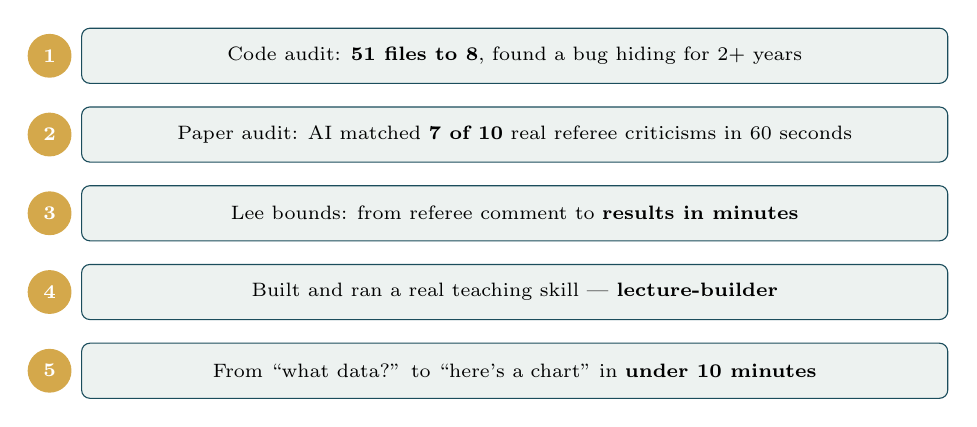
\begin{tikzpicture}[
  takeaway/.style={
    draw=SlateTeal, fill=PaleSage, rounded corners=3pt,
    minimum width=11cm, minimum height=0.7cm,
    align=center, font=\scriptsize
  }
]
  \node[circle, fill=UVMGold, text=white, font=\scriptsize\bfseries, minimum size=0.5cm] (n1) at (-6.2,2.0) {1};
  \node[takeaway, anchor=west] (t1) at (-5.8,2.0) {Code audit: \textbf{51 files to 8}, found a bug hiding for 2+ years};
  \pause
  \node[circle, fill=UVMGold, text=white, font=\scriptsize\bfseries, minimum size=0.5cm] (n2) at (-6.2,1.0) {2};
  \node[takeaway, anchor=west] (t2) at (-5.8,1.0) {Paper audit: AI matched \textbf{7 of 10} real referee criticisms in 60 seconds};
  \pause
  \node[circle, fill=UVMGold, text=white, font=\scriptsize\bfseries, minimum size=0.5cm] (n3) at (-6.2,0.0) {3};
  \node[takeaway, anchor=west] (t3) at (-5.8,0.0) {Lee bounds: from referee comment to \textbf{results in minutes}};
  \pause
  \node[circle, fill=UVMGold, text=white, font=\scriptsize\bfseries, minimum size=0.5cm] (n4) at (-6.2,-1.0) {4};
  \node[takeaway, anchor=west] (t4) at (-5.8,-1.0) {Built and ran a real teaching skill --- \textbf{lecture-builder}};
  \pause
  \node[circle, fill=UVMGold, text=white, font=\scriptsize\bfseries, minimum size=0.5cm] (n5) at (-6.2,-2.0) {5};
  \node[takeaway, anchor=west] (t5) at (-5.8,-2.0) {From ``what data?'' to ``here's a chart'' in \textbf{under 10 minutes}};
\end{tikzpicture}
\vskip8pt
\onslide<6->{%
\begin{tcolorbox}[accentbox, width=11cm, halign=center, top=3pt, bottom=3pt]
\small Six workflows. Six artifacts on disk. \textbf{All reusable.}
\end{tcolorbox}
}
\end{frame}

%% ====== SLIDE: RESOURCES ======
\begin{frame}{Resources}
\begin{columns}[T]
\begin{column}{0.47\textwidth}
\begin{tcolorbox}[keybox, title={\faLink\quad Links}]
\small
\begin{itemize}\setlength{\itemsep}{4pt}
  \item \textbf{Bootcamp website:}\\{\scriptsize\ttfamily thinkingwithagents.github.io}
  \item \textbf{Skills library:}\\{\scriptsize\ttfamily skills.sh}
  \item \textbf{Econ skills:}\\{\scriptsize\ttfamily github.com/thinkingwithagents/skills}
  \item \textbf{Claude Code docs:}\\{\scriptsize\ttfamily docs.anthropic.com/en/docs/claude-code}
\end{itemize}
\end{tcolorbox}
\end{column}
\begin{column}{0.47\textwidth}
\begin{tcolorbox}[keybox, title={\faTerminal\quad Install Commands}]
\small
\textbf{Step 1:} Install Node.js\\
{\scriptsize\ttfamily nodejs.org} $\rightarrow$ click LTS\\[4pt]
\textbf{Step 2:} Install Claude Code\\
{\scriptsize\ttfamily npm install -g @anthropic-ai/claude-code}\\[4pt]
\textbf{Step 3:} Install econ skills\\
{\scriptsize\ttfamily npx skills add thinkingwithagents/skills}\\[4pt]
\textbf{Step 4:} Launch\\
{\scriptsize\ttfamily claude}
\end{tcolorbox}
\end{column}
\end{columns}
\end{frame}

%% ====== CLOSING SLIDE: THINKING WITH AGENTS ======
{
\setbeamertemplate{footline}{}
\begin{frame}[plain]
\begin{tikzpicture}[remember picture, overlay]
  \fill[SlateTeal] (current page.north west) rectangle (current page.south east);
  \fill[UVMGold] ([yshift=0.3cm]current page.center -| current page.west) rectangle ([yshift=0.25cm]current page.center -| current page.east);
  \node[anchor=center, text=white, font=\fontsize{24}{30}\bfseries\selectfont]
    at ([yshift=2.2cm]current page.center) {Thinking With Agents};
  \node[anchor=center, text=UVMGold, font=\fontsize{14}{18}\selectfont]
    at ([yshift=1.3cm]current page.center) {Online sessions coming this summer};
  \node[anchor=center, text=white, font=\normalsize, text width=10cm, align=center]
    at ([yshift=-0.3cm]current page.center) {Workshops, deep-dives, and Q\&A on agentic AI for academic research.};
  \node[anchor=center, text=PaleSage, font=\small]
    at ([yshift=-1.7cm]current page.center) {Stay tuned for dates and registration:};
  \node[anchor=center, text=UVMGold, font=\small\ttfamily]
    at ([yshift=-2.3cm]current page.center) {thinkingwithagents.github.io};
  \node[text=white, opacity=0.04, font=\fontsize{100}{100}\selectfont, anchor=center, rotate=15]
    at ([xshift=5cm, yshift=-1cm]current page.center) {\faBrain};
\end{tikzpicture}
\end{frame}
}

\end{document}
